\chapter{Integrating structural feedback in conceptual design tools}
\label{ch:Integrating structural feedback}
In the conventional workflow, the architect uses geometric modeling tools and the engineer deploys structural analysis tools in sequential steps. Parametric modeling tools offer an improvement to this workflow, as structural analysis plug-ins are available. This allows the user to obtain structural feedback earlier in the design phase, but still as a sequential step to the geometric modeling. The present work aims to improve the workflow by integrating structural feedback with geometric modeling. However, this creates new demands on conceptual design tools. 

\section{Human--computer interaction}
Conceptual design tools should inspire and encourage users to explore design alternatives. This places demands on the human--computer interaction of such tools. The tools need to be interactive and allow users to quickly create new models, or to make changes to existing models. 

Direct manipulation is a human--computer interaction style that enables users to directly manipulate objects on the screen. By doing so, the perceptual and cognitive resources required to understand and operate the user interface are reduced. Paper A describes a conceptual design tool that employs a very direct manipulation style in a user interface for 2D models. This style is achieved by taking advantage of a multi-touch screen, which literally closes the gap between the human and the computer. Using this tool, users can input a structural model using gestures similar to those found in drawing applications for tablets (see Figure \ref{fig:interaction}). This allows users to quickly explore different design alternatives.

\begin{figure}
  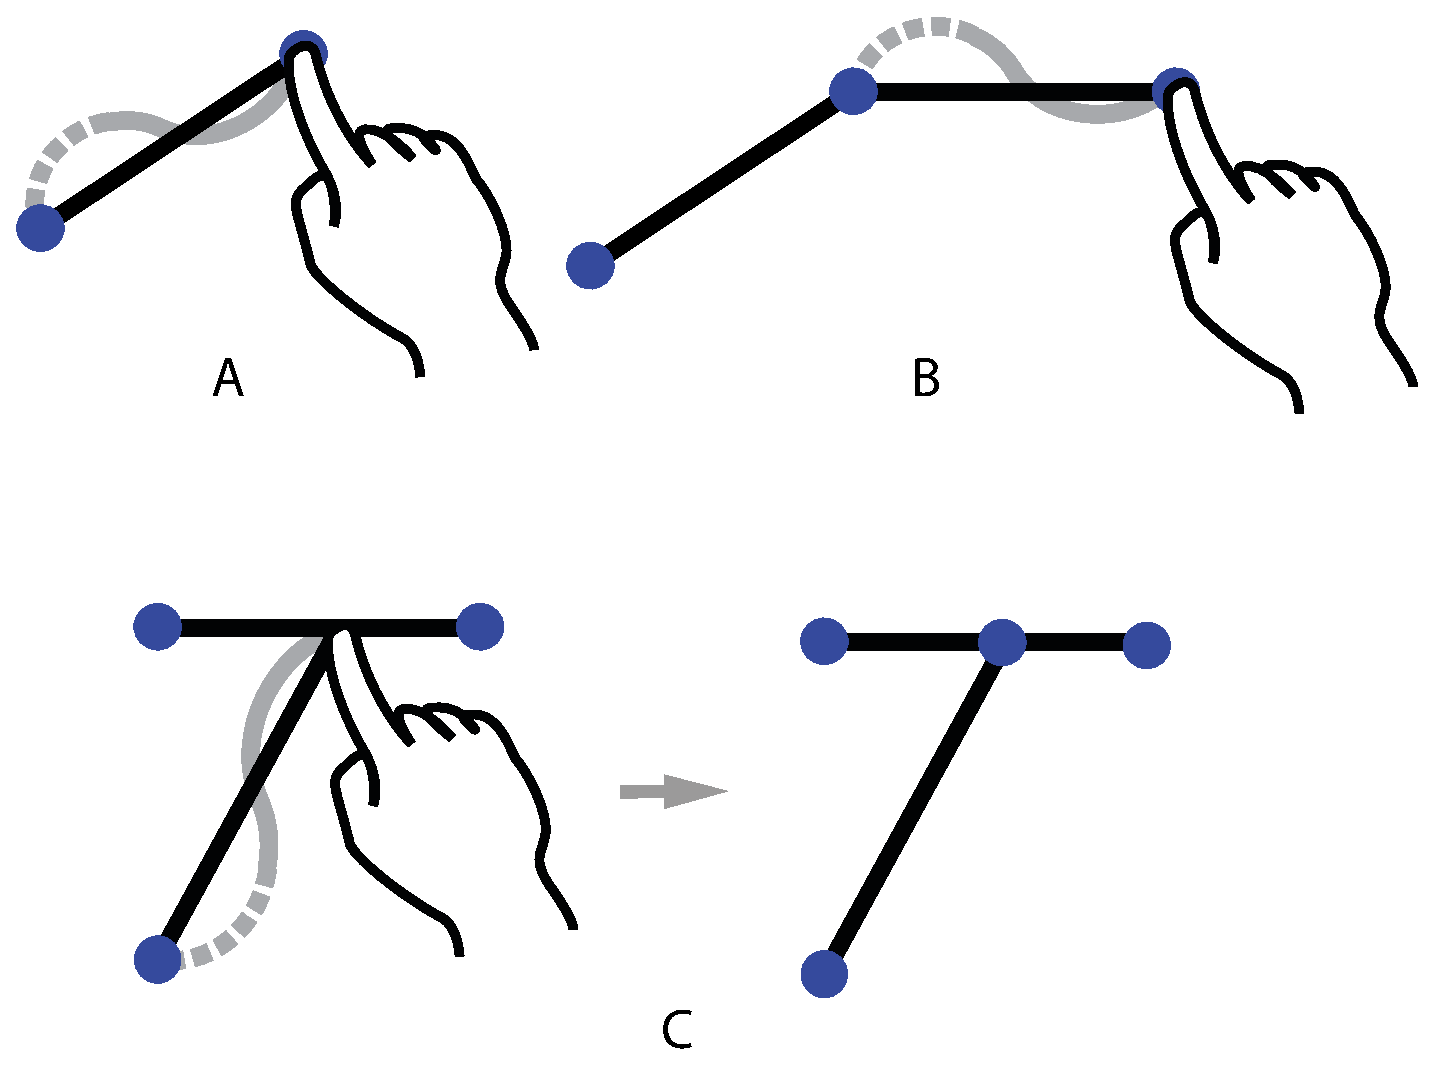
\includegraphics[width=330pt]{graphics/interaction.eps}
  \caption{Modeling gestures in the developed application, Sketch a Frame}
  \label{fig:interaction}
\end{figure}

Achieving a very direct manipulation style in 3D has been made possible by the emergence of new 3D input controllers. This creates an opportunity to create conceptual design tools with a very direct manipulation style for 3D. In Paper B , this opportunity has been explored where a developed conceptual design tool that employs a 3D input controller named the Leap Motion Controller is presented. 

In Paper A, a very direct manipulation cycle is proposed to further improve the interactivity of the user interface in conceptual design applications. As the user is modeling, computations are continuously performed, and the result is automatically visualized once the modeled structure is in static equilibrium. This removes the need for a specific ``compute step,’’ and further integrates structural feedback into the geometric modeling. This direct manipulation cycle is also employed in the application developed in Paper B.

\section{Structural feedback}
To integrate structural feedback into conceptual design applications, structural analysis must be integrated into the geometrical modeling phase. The feedback should be easy to understand and provide valuable information about the structural behavior and performance of the design.

\begin{figure}
  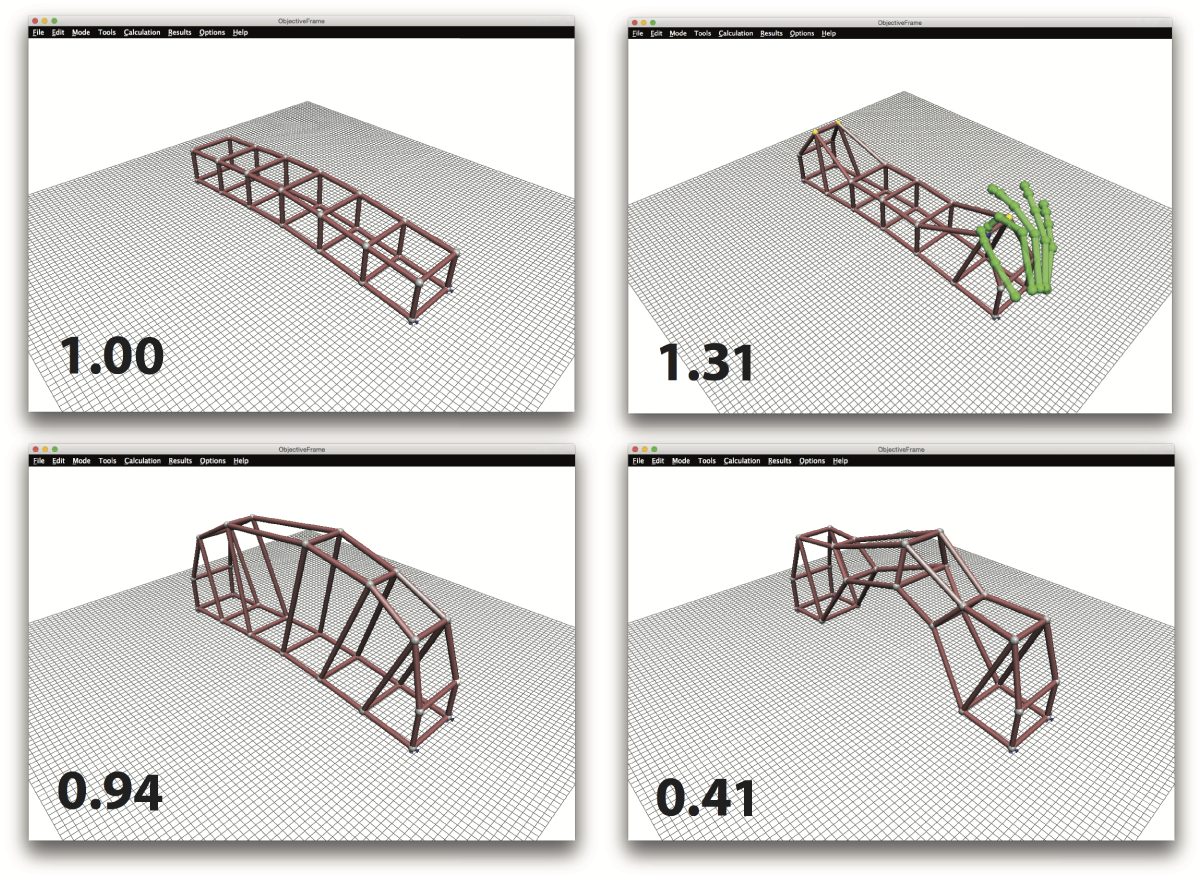
\includegraphics[width=350pt]{graphics/performance-feedbacku.png}
  \caption{Geometric modeling with real-time performance index}
  \label{fig:performance-feedback}
\end{figure}

In the applications developed in Papers A and B, an external force can be applied to the modeled structure. If the model is in static equilibrium, the resulting deformations can be visualized in real time. The user can then adjust the forces using direct manipulation, and observe in real time how the structural deformation responds. In Paper A, when an external force is applied, the resulting normal forces and the moment envelope can also be visualized in real time. This can improve the user’s understanding of how the structure responds to external forces, how stresses propagate through the different members, and the stiffness of the structure in different directions.

The structural feedback should be easy to understand. In Paper B, the model is manipulated by the previously described direct manipulation methods, and users are simultaneously presented with a performance index that measures how well the structure is performing. This performance index is the normalized strain energy of the model; thus, a lower number corresponds to a better-performing structure (see Figure \ref{fig:performance-feedback}). Using a single value to represent the performance of a structure makes it easy for users to understand how geometrical modifications affect the structural performance.


\section{Structural optimization}
Integrating structural optimization into conceptual structural design has the possibility to not only provide feedback about the structural performance, but also to guide the user towards geometries that are structurally sound. 

A genetic algorithm for shape optimization is implemented in the application described in Paper A. Users first select which nodes can be moved by the optimizer and in which direction (vertical or horizontal) they can be moved. The optimization is then executed to minimize the strain energy. Once the analysis is complete, the best-performing structure is visualized (see Figure \ref{fig:ipad-ga}). 

\begin{figure}
  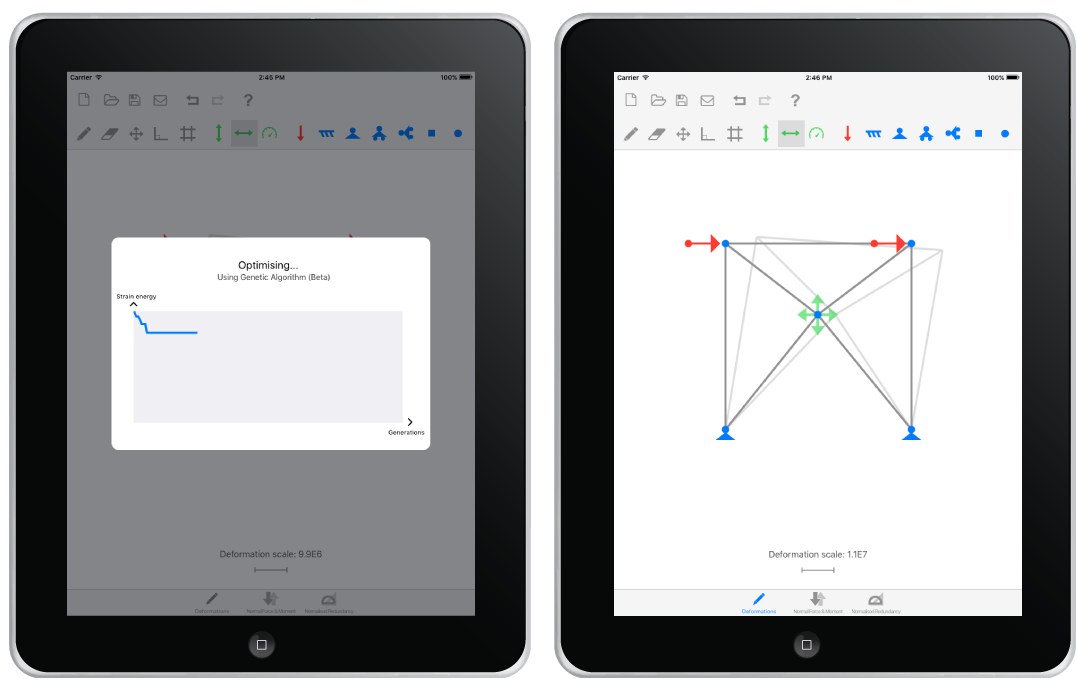
\includegraphics[width=330pt]{graphics/ipad-ga.png}
  \caption{Genetic algorithm optimization in Sketch a Frame}
  \label{fig:ipad-ga}
\end{figure}

Form-finding can be used to identify the static equilibrium for a structure under load. In Paper B, the dynamic relaxation method is implemented to enable form-finding in an interactive 3D environment. Users can further explore the form-found structure by applying and manipulating an external force. A point load can be used to move away from the optimal solution in order to find other interesting sub-optimal solutions that might be more aesthetically attractive. The point load can also, for example, represent a supporting column or a hanging installation in the structure.


\section{Visual representations}
After structural analysis computations have been performed, the result can be visualized. For conceptual structural design tools, visualization should ideally allow users to understand the results quickly. One such example is graphic statics, which visualizes forces as line lengths in a force diagram. Compared to using colors to represent the magnitude of the forces, this is beneficial to users’ understanding as it removes a layer of abstraction. Users can immediately understand the magnitude of the forces without the need for any form of colorbar.

Dynamic behavior can be visualized using animations, as in the application developed in Paper A. If a force is applied to a model which is not in static equilibrium, the resulting rigid body motion is visualized using an animation. This allows users to quickly understand that the model is not in static equilibrium, and how it needs to be modified in order to be in static equilibrium.

\subsection{Example - Stress lines}
The structural behavior of 1D elements, such as bar and beam elements, is easier to understand than that of higher-dimensional elements. Higher-dimensional elements have a more complex structural behavior. For 2D structural elements, the internal stresses can be computed and used to compute lines representing how the external load flows through the structure towards the boundaries, see Figure \ref{fig:stresslines}. In the Z-direction, this can be described as \cite{Fonseca1997}:

\begin{equation*}
\frac{\delta \tau_{xz}}{\delta x} + \frac{\delta \tau_{yz}}{\delta y} + \frac{\delta \sigma_{z}}{\delta z}= 0
\end{equation*}

The author  has explored how stress lines can be extended into 3D using volumetric elements.  The idea for the algorithm and the results are shown in Figure \ref{fig:flowlines-exp}. Volumetric elements are colored according to the von Mises stress, and the green dots denote boundary conditions. However, this method has some drawbacks: it is not clear how to interpret the lines, the results are sensitive to the mesh size, and the computational load is significant. Additionally, only the internal stresses acting in the Z-direction are considered here.

Although, the method described here have to be developed further. There is a need for developing better methods for visualizing results in more complex situations.

\begin{figure}
  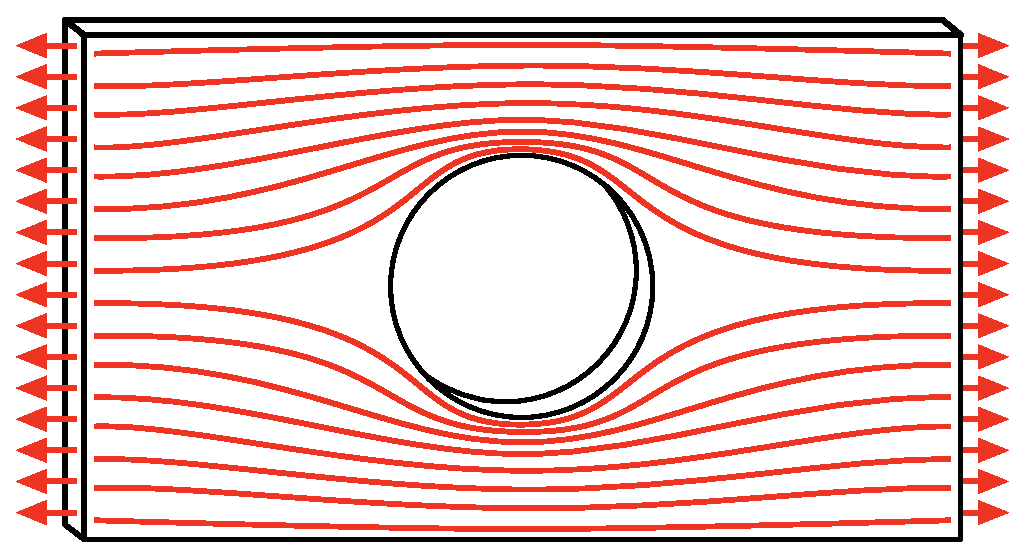
\includegraphics[width=230pt]{graphics/stresslines.eps}
  \caption{Stress lines for a 2D problem}
  \label{fig:stresslines}
\end{figure}
 
\begin{figure}
  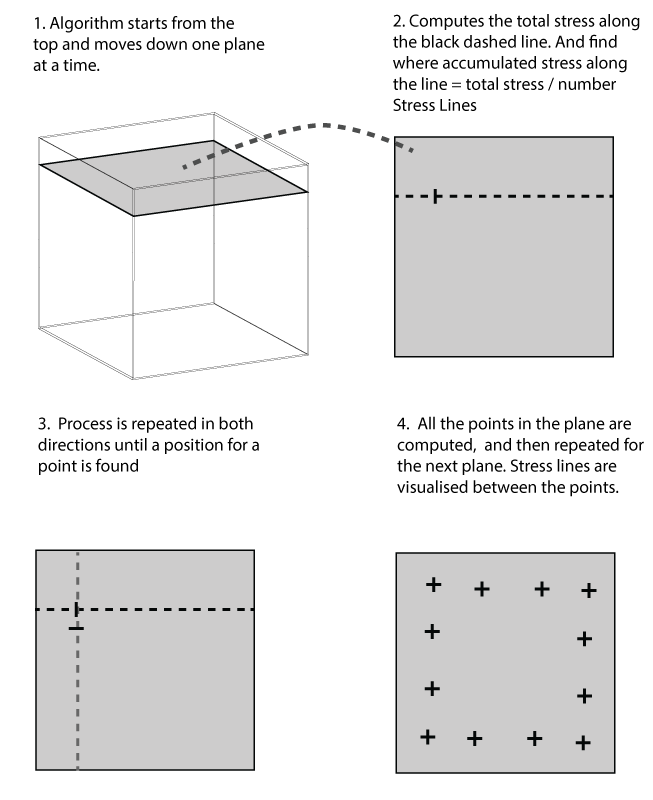
\includegraphics[width=360pt]{graphics/flowlines-exp.eps}
  \caption{Computing stress lines for 3D}
  \label{fig:flowlines-exp}
\end{figure}
